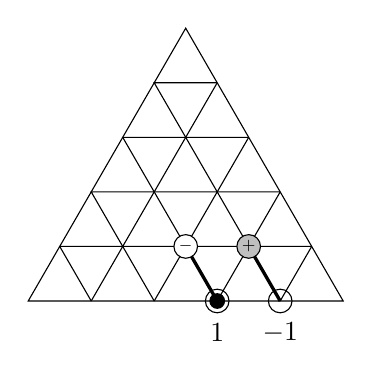
\begin{tikzpicture}[baseline=0cm]
\draw (0,0) -- (4,0) -- (60:4) -- cycle;

\foreach \x in {0.8,1.6,2.4,3.2}
\draw (4,0)++(120:\x) edge (4-\x,0) -- (60:\x) -- (\x,0);

\draw[very thick] (2.4,0) -- +(120:0.8) (3.2,0) -- +(120:0.8);

\fill (2.4,0) coordinate(v) circle[radius=0.1];% ++(0,-0.4)node{$v$};
\foreach \x in {2.4,3.2}
\draw (\x,0) circle[radius=0.15];
\draw (2.4,-0.4)node{$1$} (3.2,-0.4)node{$-1$};

\draw[fill=white] (v) ++(120:0.8)node{\tiny$-$} circle[radius=0.15];
\draw[fill=lightgray] (v) ++(60:0.8)node{\tiny$+$} circle[radius=0.15];
\end{tikzpicture}